%Projekt pro p�edm�t ITY
%Autor: Miroslav Pavelek- 1BIT
%Datum:	23. - 24.2.2012
\documentclass[11pt,a4paper,titlepage]{article}
\usepackage[czech]{babel}
\usepackage[utf8]{inputenc}
\usepackage{times}
\usepackage[left=2cm,text={17cm,24cm},top=2.5cm]{geometry}
\usepackage[bookmarks=true,pdfborder={0 0 0}]{hyperref}
\usepackage{graphicx}
\usepackage[font={small,it}]{caption}
\usepackage[T1]{fontenc}
%uvozovky
\providecommand{\uv}[1]{\quotedblbase #1\textquotedblleft}

\begin{document}

\begin{titlepage}
\begin{center}
{\Huge\textsc{Vysoké učení technické v~Brně}}\\
\medskip
{\huge\textsc{Fakulta informačních technologií}}\\
\vspace{\stretch{0.382}}
{\LARGE Praktické aspekty vývoje software\,--\,3.\,projekt}\\
\medskip
{\Huge Uživatelská příručka}\\ 
\vspace{\stretch{0.218}}
%%\begin{minipage}{\linewidth}
%%\makebox[\linewidth]{%    
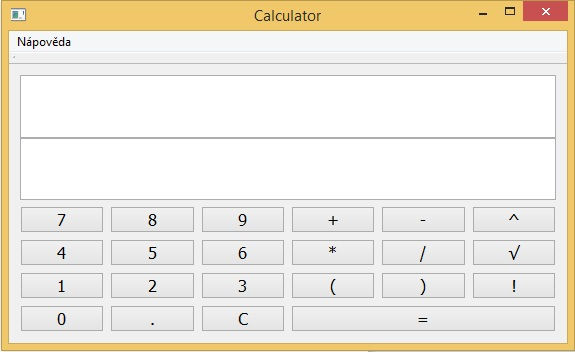
\includegraphics[keepaspectratio=true,scale=0.6]{mainPicture} \\
%%\end{minipage}
\vspace{\stretch{0.618}}
{\Large Miroslav Pavelek, Ivan Ševčík, Tomáš Polešovský, Zdeněk Sklenář}
\end{center}
\end{titlepage}
%% Obsah
\tableofcontents
\pagebreak

%Reálný text
\section{Úvod}
V této příručce je popsáno ovládaní a funkce kalkulačky, která byla vytvářena do předmětu Praktické aspekty vývoje software. Příručka je koncipována tak, že se uživatel nejprve seznámí s funkcemi programu, poté s jeho ovládacími prvky a nakonec s instalací a odinstalací programu.
\section{Charakteristika programu}
Kalkulačka zvládá základní matematické operace - sčítání, odčítání, násobení a dělení. Kromě toho zvládá i faktoriál, umocňování s přirozenými exponenty a odmocňování. Dále jsou zde zabudované závorky, které určují prioritu operací.\\
\textbf{Podporované systémy:} Microsoft Windows XP a vyšší
\section{Ovládací prvky programu}
Uživatelské rozhraní se skládá ze dvou částí - z klávesnice a displeje. \\ \\
\noindent%
\begin{minipage}{\linewidth}
\makebox[\linewidth]{%    
  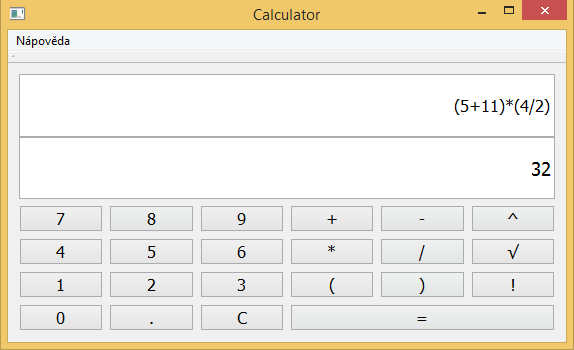
\includegraphics[keepaspectratio=true,scale=0.6]{example}}
  \label{obr1}
\captionof{figure}{Uživatelské rozhraní }\label{obr1}
\end{minipage}
\subsection{Klávesnice}
Na klávesnici (sekce 1 na obrázku \ref{obr1}) jsou umístěné tlačítka číslic, základních matematických operací a tlačítko „C“, které vyčistí displej. Po zmáčknutí tlačítek se objeví jejich příslušný ekvivalent (např. \emph{sqrt()} v případě odmocniny nebo \emph{fact()} v případě faktoriálu) na displeji.
\subsection{Displej}
Displej je složen ze dvou řádků. Na prvním z nich se zobrazují čísla a znaky, které zadal uživatel pomocí numerické klávesnice nebo stisknutím dostupných tlačítek. Na druhém řádku lze po stiknutí klávesy „Enter“,nebo po zmáčknutí tlačítka „=“ vidět výsledek.
Výsledek je vypisován na 6. desetinných míst, s tím že poslední desetinné místo je zaokrouhlené.
\section{Instalace programu}
\subsection{Instalace pomocí instalátoru}
Kalkulačka jde nainstalovat pomocí instalatoru \emph{instalator.msi}, který je umístěn ve zdrojové složce.
 \textbf{Pozor:} Tento způsob instalace vyžaduje práva administrátora.
\begin{enumerate}
  \item Spustíme soubor \emph{instalator.msi}
  \item Klikneme na \underline{Next >}
  \item Vybereme umístění, kde chceme nainstalovat kalkulačku a klikneme na \underline{Next >}
  \item Poté klikneme na \underline{Install}. Tímto se aplikace začne instalovat.
  \item Po instalaci se zobrazí poslední obrazovka, na které stačí kliknout na \underline{Finish}. 
\end{enumerate}
Aplikaci jde poté spustit pomocí zástupce \emph{Calculator}, který je umístěn na ploše.
\subsection{Manuální instalace}
Druhou možností je instalace programu pomocí samorozbalovacího archivu \emph{Calculator.sfx.exe}. Po spuštění stačí pouze vybrat cestu, do které se ma program instalovat a kliknout na „Extract“.
\textbf{Pozor:} Tento způsob instalace nevytváří zástupce aplikace, v případě potřeby si jej uživatel musí vytvořit sám.
\section{Odinstalace programu}
\subsection{Odinstalování automatické instalace}
Pokud byl prográm nainstalován pomocí instalátoru, tak existují dva způsoby odinstalace programu.
\subsubsection{Odinstalování přes instalátor}
\begin{enumerate}
  \item Spustíme soubor \emph{instalator.msi}, kterým jsme nainstalovali kalkulačku.
  \item Klikneme na \underline{Next >}
  \item Klikneme na \underline{Remove}.
  \item Na další obrazovce opět klikneme na \underline{Remove}.
  \item Po odinstalaci se zobrazí poslední obrazovka, na které stačí kliknout na \underline{Finish}. 
\end{enumerate}
\subsubsection{Odinstalace přes Ovládací panely}
\begin{enumerate}
  \item Spustíme \underline{Ovládací panely} (např. pomocí zmáčknutí kombinace kláves win + R, kde stačí napsat „control“ a spustit)
  \item Zde vybereme \underline{Přidat nebo odebrat programy}, popřípadě \underline{Odebrat Program}.
  \item Zde najdeme položku \underline{Calculator} a označíme ji.
  \item Klikneme na \underline{Odinstalovat}.
  \item Potvrdíme odinstalaci v instalátoru.
  \end{enumerate}
\subsection{Manuální odinstalace programu}
Pokud jste program instalovali manuálně pomocí samorozbalovací archivu \emph{Calculator.sfx.exe}, tak stačí pouze smazat složku, do které jste program rozbalili.
\section{Kontakt}
V případě nejasností nebo přípomínek se můžete obrátit na e-mailovou adresu vedoucího projektu na adrese \emph{\href{mailto:xpoles05@stud.fit.vutbr.cz}{xpoles05@stud.fit.vutbr.cz}}.
\end{document}

